\documentclass[12pt]{article}
\usepackage[a4paper, total={6in, 8in}]{geometry}
\usepackage[utf8]{inputenc}
\usepackage[english]{babel}
\usepackage{titlesec}
\usepackage{graphicx}
 

\usepackage{setspace}
\doublespacing


%   Thesis / research paper title.
%	Student name, student number.
%	Date.
%	Keywords: 2 on concepts, 2 on methods, 1 on the field of observation.
%	Department, University.


\title{ }
\author{Berthin Bitja \\ 4532321}
\date{}



\usepackage[
style=nature,
date=year,
backend=biber,
natbib=true,
doi=false,
defernumbers=true
]{biblatex}

\addbibresource{bib-influenza.bib}

\begin{document}

\begin{titlepage}
	\centering

	{\Large\bfseries Deep learning approaches for forecasting the global spread influenza \par}
	\vspace{2cm}
	{\small Berthin Bitja \\ 4532321 \par}
	{\small \today\par}
	\vfill
	
	{\large Department of Biology \\ University of Ottawa \par}

% Bottom of the page

\end{titlepage}

\newpage

\tableofcontents

\newpage

\section{Background}
Influenza is a recurrent public health problem. The virus infects approximately 5 to 10 \% of the global adult population and 20 to 30 \% of children every year causing respiratory illness and complications\autocite{Ting2017}. In Canada, the total cost of each influenza season is estimated to 1 billion per year\autocite{Molinari2007}. Virus re-assortment (i.e. mixing of gene segments of multiple viruses) and the accumulation of mutations contribute to the emergence of new influenza virus variants. However, most of these variants do not have the ability to spread among humans and subsequently cause a pandemic. Immunization programs have been developed by public health agencies and government to reduce the effects of the circulating strains by preventing infection and widespread transmission\autocite{Jefferson2005}. 

In order for those programs to be efficient the scientific community developed predictive approaches such as time-series models, method of analogs, compartmental models, agent-based models or metapopulation models\autocite{nsoesie2014}. For instance, “GLEaMviz” is a publicly available software that simulates the spread of emerging human-to-human infectious diseases across the world. The simulation engine uses a stochastic computational scheme that integrates worldwide high-resolution of human demographic and mobility data to simulate disease spread on the global scale. The detailed mobility networks used in GLEaMviz design enable description of the diffusion pattern of the ongoing epidemic\autocite{Broeck2011}. This model is used to visualize the geo-temporal evolution of influenza epidemics. One major difficulty in applying forcasting models for influenza is the limited assumptions under which they operate, combined with the limitations on the knowledge we have on human behavior. Although, the GLEaMviz design provides insights on influenza spread, producing reliable predictions during an outbreak remains a challenge.

Disease transmission is a complex spatio-temporal process. It includes environment factors\autocite{Pica2012} such as temperatures, humidity or pressure, genomic information such as drug resistant mutations, and human behavior that can be represented by airport traffic. In addition, these type an of data constitute large datasets. In this context, Deep learning (DL) offers an intuitive  approach to resolve prediction problems by enabling computational models that are composed of multiple processing layers based on neural networks to learn representations of data with multiple levels of abstraction  \autocite{Lecon2015, Miotto2017}. Those "black boxes" reduce the need for feature engineering considering that features are learned from data. Despite, being used in various fields such as speech recognition, visual object recognition, object detection, drug discovery and genomics, there are no publicly available tools implementing these algorithms for the forecasting of influenza outbreaks.

\section{Reasearch Question}

The goal of this thesis is to implement a DL system to predict influenza outbreak at the local, regional, national, or global level. This thesis has three aims. The first aim is (i) to design the architecture of a deep neural network integrating mobility data, genomic data and environmental data to predict common epidemic measures \autocite{nsoesie2014} including locations,  duration's, activity of the different type and subtypes of influenza. The second aim is (ii) to develop a pipeline to automate the process of data retrieval. The final aim is (iii) to assess the overall performance of our design. The motivation of this research is to expand the knowledge on predictive methods based on DL approaches for surveillance and forecasting of infectious diseases and explores the relevance of using DL in application to influenza forecasting. 

\section{Data}
 
 Influenza transmission is affected by a number of factors, including environmental determinants, host behavior, host defense mechanisms, and virus infectivity\autocite{Pica2012}. In order to process the data we need to create a specific profile for each type and/or subtype of Influenza virus. As a result, we need to create a pipeline to merge different type of datasets such as Influenza Virus Database\autocite{chang2006influenza} for genetic determinant, Global Surface Summary of the Day (GSOD)\autocite{Lott1998} database for environmental determinants, FluNet database\autocite{flahault1998} for virus infectivity and the Bureau of Transportation Statistics database\autocite{mcdonald2013} for host behavior.

Influenza Virus Database\autocite{IVD-fb} contains nucleotide sequences from samples all over the world. The influenza Virus database includes meta-data for each sequence such as the length of sequence, the host, protein, sub-type, country, region, date, virus name and  drug resistant mutation. 

The climatic data is obtained from the USAF Climatology Center, located in the Federal Climate Complex with National Climatic Data Center (NCDCI)\autocite{Lott1998}. The parameters included for each station are : id of the station, country, longitude and latitude, elevation, mean temperature, mean dew point, mean sea level pressure, mean station pressure, mean visibility, mean wind speed, maximum sustained wind speed, maximum wind gust, maximum temperature, minimum temperature, precipitation amount, snow depth and indicator for occurrence of fog, rain or drizzle, snow or ice pellets, hail, thunder, tornado/funnel cloud.

The epidemic dataset is provided by FluNet\autocite{flahault1998}. A global tool for influenza virological surveillance launched in 1997  by WHO's Global Influenza Surveillance and Response System (GISRS). The virological data entered into include the Influenza-Like Country, area or territory, Illness (ILI) activity, time and number of influenza viruses detected by subtype.

The Bureau of Transportation Statistics provide air traffic data on international market. The dataset includes carrier's name, origin, destination, aircraft type and service class for transported passengers, freight and mail, available capacity, scheduled departures and departures performed. Flights with both origin and destination in a country outside the U.S are not included.

\section{Methodology}

\begin{figure}[h]
    \centering
    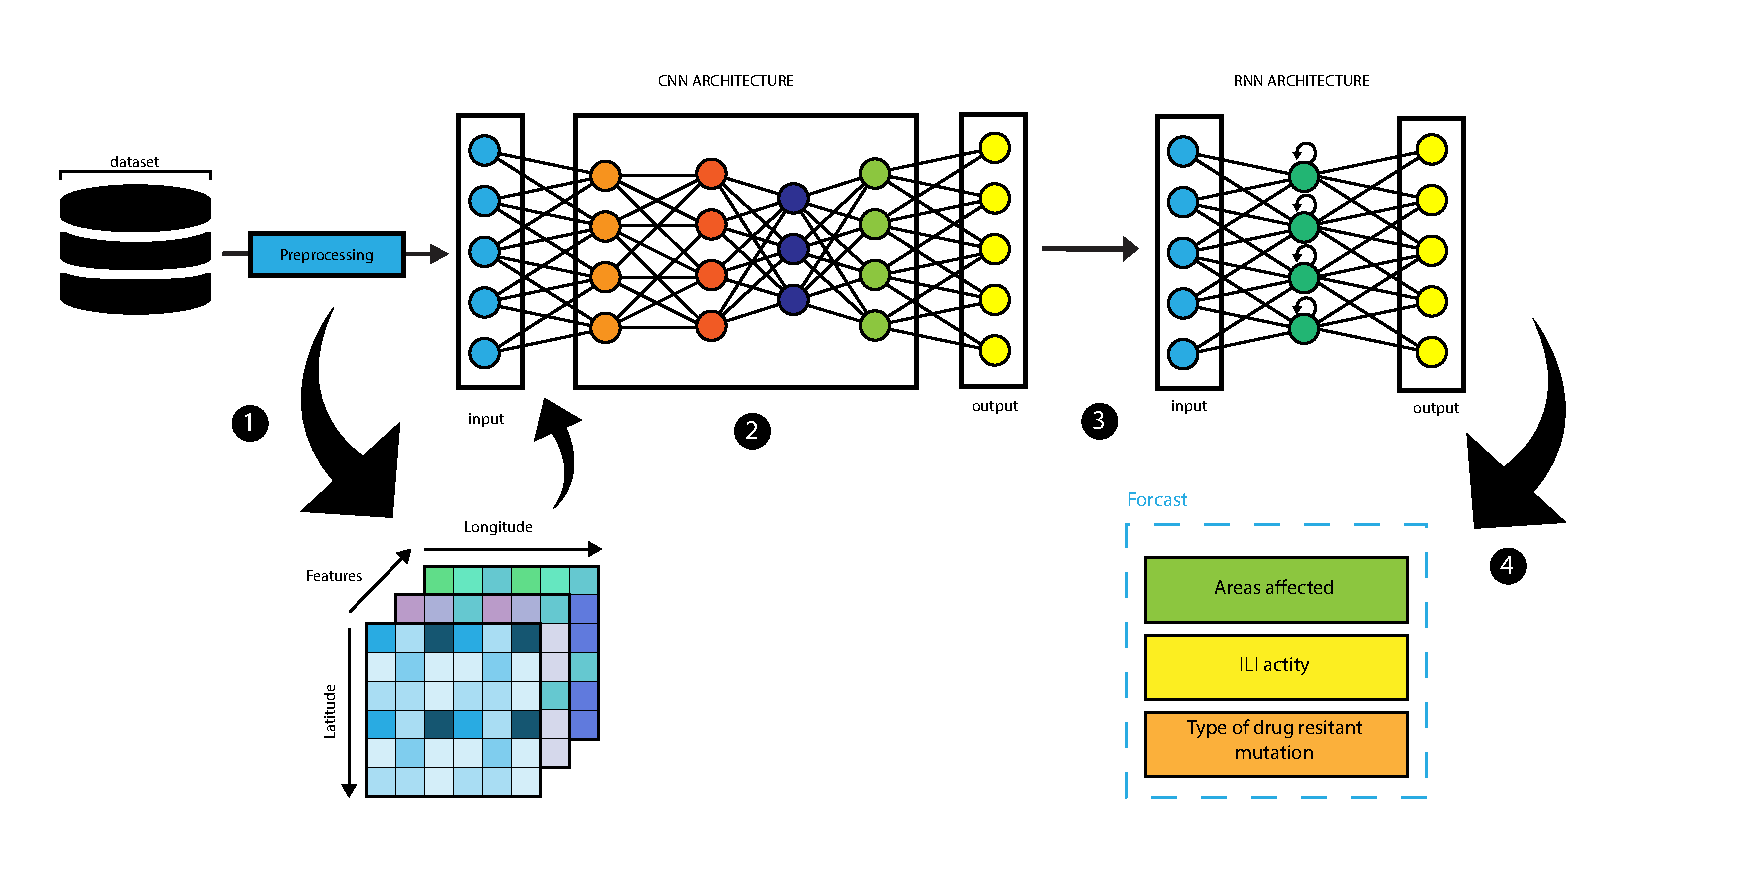
\includegraphics[width=\textwidth]{figure-1.png}
    \caption{ Illustration of the Proposed Methodology}
    \label{fig:mesh1}
\end{figure}

To achieve the objectives illustrated in figure \ref{fig:mesh1} we define for each class of virus a profile based on geographic, climatic,  genetic parameters and mobility data. There's essentially 4 steps we need to complete achieve our objectives, define the neural network architecture, implement the neural network, fit the neural network and evaluate the neural network.

The problem can be represented as Hidden Markov Models (HMMs), see figure \ref{fig:RNN}. We define a profile for the virus, $p$, that varies trough discrete time step, $t$, to give an output or an observation, $o$. The state, $s$, of the system is defined by : 
$$s_t = f(Up_t+ Ws_{t-1})$$ where $(U,W)$ are parameters of the system. The function $f$ usually is a non-linear function that transform the input from the previous layer to a new output for the next layer. This function is called an activation function. Each observations, $o_{t=0,1,2 ... }$ depends on the computed knowledge we have on the profile of the virus. The prediction or observations, $o_t$, can be produced trough a vector of probabilities  $$o_t=softmax(Vs_t)$$, where, $V$, represent the features of our virus profile. $Softmax$ function calculates the probabilities distribution of an event over ‘n’ different events. 
The type of neural networks to compute this class of problems are Recurrent Neural Networks (RNNs), see figure \ref{fig:RNN}. They perform the same task for every element of a sequence, with the output being dependant on the previous computations. In RNNs, the hidden state, $s_t$, represent "the memory" of the network. 
Finally, we will define the architecture of our neural network as multiple layer of RNNs, to analyze patterns trough week, months and/or years. 

\begin{figure}[h]
    \centering
    \includegraphics[width=\textwidth]{figure-3.png}
    \caption{ An unrolled recurrent neural network }
    \label{fig:RNN}
\end{figure}

The second step will be to implement different neural network architectures using Tensorflow as the framework. This is an open source library for fast numerical computing. This framework will allows us to build efficient series of matrix transforms in a format intended to be executed on GPU or CPU. Also, we will need define an optimization scheme to train our network. It will result in  determining parameters such as which optimization algorithm to use to train the network and the loss function\autocite{LeCun2015}.

The third step will be to fit the neural network. It signifies that we will train the model to update the weights on a training dataset. Consequently, we will need to transform the training data as matrix of input $x$ and an array of matching output patterns $y$. Then we will train the network using a backpropagation algorithm\autocite{LeCun2015} and update our weights according to the optimization algorithm and loss function.
A backpropagation algorithm requires that the network be trained for a number of epochs against the training dataset. We will divide each training period into groups of input-output pattern pairs. Thus, this will define the number of patterns that the network is exposed to before the weights are updated within an epoch.

Finaly, once our model is trained, we will implement two methods that uses historical data to assess its performance. The first backtesting method is Multiple Train-Test Splits. We will split time series into a train and test sets multiple times. This will train separately multiple model using multiple train-test splits, and will produce an accurate estimate of the performance of the models on unseen data. The second method is the Walk-Forward Validation or Rolling Window Analysis. The model will retrains as new data becomes available. To use this method we will define a minimum number of observations to train the model. Then, we will train the model on all available data or only on the most recent observations.

\section{Timescale }

\begin{figure}[h]
    \centering
    \includegraphics[width=\textwidth]{figure-2.png}
    \caption{ Proposed timeline}
    \label{fig:timeline}
\end{figure}

The time line for the completion of the project is described on the figure \ref{fig:timeline}. The first stage of the research  will be to produce a working prototype by the end of November. A time consuming step will be to automate the system, in order to automatically feed our system with the right data input. Additionaly, it will take about a month or two to train the different models. Therefore, a good trained model will be ready by the end of December. We will write the thesis methods and analysis while implementing our models. As a result, we expect that by the end of February, we will have completed the Rolling Window Analysis. Around the same time, The first draft of the thesis should be ready. We will have to finalize the discussion and conclusion of the thesis. By May, we will be submitting articles to Scientific paper. 
\newpage

\section{Discussion}

This research opens doors to a more intuitive and automated method to analyze big data in the context of epidemiology. Reliable forecasts of influenza measures will inform health care practitioners on when to expect changes. Professionals could prepare for surges in influenza cases by developing more efficient vaccines and antiviral treatments and mobilizing essential personnel (such as nurses and doctors).

The key advantages of deep learning models are robust, generalizable and scalable. The model automatically learns the most relevant features and takes in account natural variations of the data. In addition, the model design can be applied for other types of problems in different fields. Finally, the performance improves with the amount of data\autocite{LeCun2015} and processing power available (GPUs or CPUs).

Although, there are limitation associated with DL methods. Foremost, these approaches require large datasets to run. Secondly, like the human brain neural networks can becomes bias, based on their "knowledge" of the data. Lastly, it is difficult to understand to understand the behavior of deep neural networks\autocite{Miotto2017}.

In near a future, we want to build a simple user interface for the non-expert to visualize and interact with our prediction. The tool will be presented as a client-server model, where all heavy tasks are run by the server. The users will have the possibility to display the results in the form of raw data (table) or transform data (maps, charts or reports).

\printbibliography[title={Bibliography},nottype=misc,resetnumbers=true]

\end{document}
